\documentclass{article}
\usepackage[utf8]{inputenc}
\usepackage{biblatex} 
\usepackage{amsmath}
\usepackage{amsfonts}
\usepackage{amssymb}
\usepackage{amsthm}
\usepackage{graphicx}
\usepackage{array}
\usepackage{multirow}
\usepackage{booktabs}
\usepackage{subfig}

%\usepackage[margin=1.7in]{geometry}


\addbibresource{report.bib}
\bibliography{report.bib}
\usepackage[nottoc]{tocbibind}

\usepackage[skip=6pt plus1pt, indent=20pt]{parskip}


\newtheorem{theorem}{Theorem}[section]
\newtheorem{defn}[theorem]{Definition} 
\newtheorem{cor}[theorem]{Corollary}
\newtheorem{alg}[theorem]{Algorithm}
\newtheorem{example}[theorem]{Example}
\newtheorem{lemma}[theorem]{Lemma}
\newtheorem{prop}[theorem]{Proposition}

\title{Understanding the Behaviour of Reinforcement Learning Agents in Cyber Defence; Conclusions and Reflections}
\author{Hannah Harrison }
\date{August 2023}


\begin{document}

\maketitle

\vspace{1cm}
\begin{center}
    

\noindent Part of a dissertation project submitted to the University of Bristol in accordance with the requirements for award of the degree of MSc Mathematics of Cybersecurity in the Faculty of Science.

\end{center}

\newpage

\vspace{8cm}
\begin{center}
  \textbf{ \Large Declaration of Authorship}
  \vspace{0.5cm}

I declare that the work in this dissertation was carried out in accordance with the Regulations of the University of Bristol. The work is original, except where indicated by special reference in the text, and no part of the dissertation has been submitted for any other academic award. For all ideas taken from other sources (books, articles, internet), the source of the ideas is mentioned in the main text and fully referenced at the end of the report. All material which is quoted essentially word-for-word from other sources is given in quotation marks and referenced. Pictures and diagrams copied from the internet or other sources are labelled with a reference to the web page or book, article etc. Any views expressed in the dissertation are those of the author.


\end{center}




\newpage



\newpage 

\tableofcontents
\pagebreak

%Then feel free to be more "out there" in the individual writeup, discussing the technical issues, any blind alleys, what worked and didn't, etc
% separate out in your mind the “methods” and the “reflections” part.

\section{Introduction}
This paper acts as a companion to the technical report entitled `Understanding the Behaviour of Deep Reinforcement Learning Agents in Cyber Defence'. Motivated by the increasing popularity of fundamentally incomprehensible DeepRL agents within the field of cyber defence, this research project presents a causal explanation generation mechanism tailored to the setting of the novel cybersimulator YAWNING TITAN \cite{inproceedings} (abreviated YT). The aim of this supplementary report is to provide insight into the challenges faced during this research, as well as to justify the decisions made, evaluate how the project met the intended goals and discuss what could have been done differently. To this end, this report is structured as follows. In Section 2, I will briefly reflect on the project aims and the extent to which they were achieved. In Section 3, I will discuss the three main phases of the research, and review the challenges faced during each. Finally, I will conclude by considering the limitations of the research, and explain the further work I would undertake, given more time. 

\section{Project aims}

As laid out in the preparation report, there were three main aims for this project;

\begin{enumerate}
    \item To explore the use of reinforcement learning (RL) in simulated networks, and develop a reinforcement learner which can defend against simple attacks.
    \item To survey the application of causal models for  providing explanations for reinforcement learning.
    \item To develop a proof of concept which utilises a causal model to explain the decisions made by the developed reinforcement learner. 
\end{enumerate}

\noindent Overall, the project was successful in all three aims; Section 3 of the technical report provides a detailed review of the current state of explainable reinforcement learning (XRL) and Section 5 a working proof of concept using a causal model to provide insight into the decisions made by a DeepRL agent trained in the YT scenario. However, as will be discussed in Section 4 of this report, only a very specific, simplified scenario within YT was considered. Thus there is much room for extension and indeed much need for it in order for the method proposed to be of use in a wider variety of network defence scenarios.  


\section{Discussion} 
%Go through what I did and how it fit/ didnt fit the plan
% Gantt chart, things did actually go to plan

In line with the aims outlined in Section 2, my research was divided into three main phases; first I researched reinforcement learning and implemented a learner within the YT environment, before reviewing the literature around causal XRL and finally developing such a method for the YT scenario. The timeline for the project was set out as in the Gantt chart in Figure \ref{fig:gantt} and, due to keeping a detailed log and frequently referring to the plan, the project progressed almost exactly as expected, with the exception of the proof of concept development taking slightly longer than expected. This was due to challenges faced within the YT environment, which will be discussed further in Section 3.3.

\begin{figure}[htp]
    \centering
    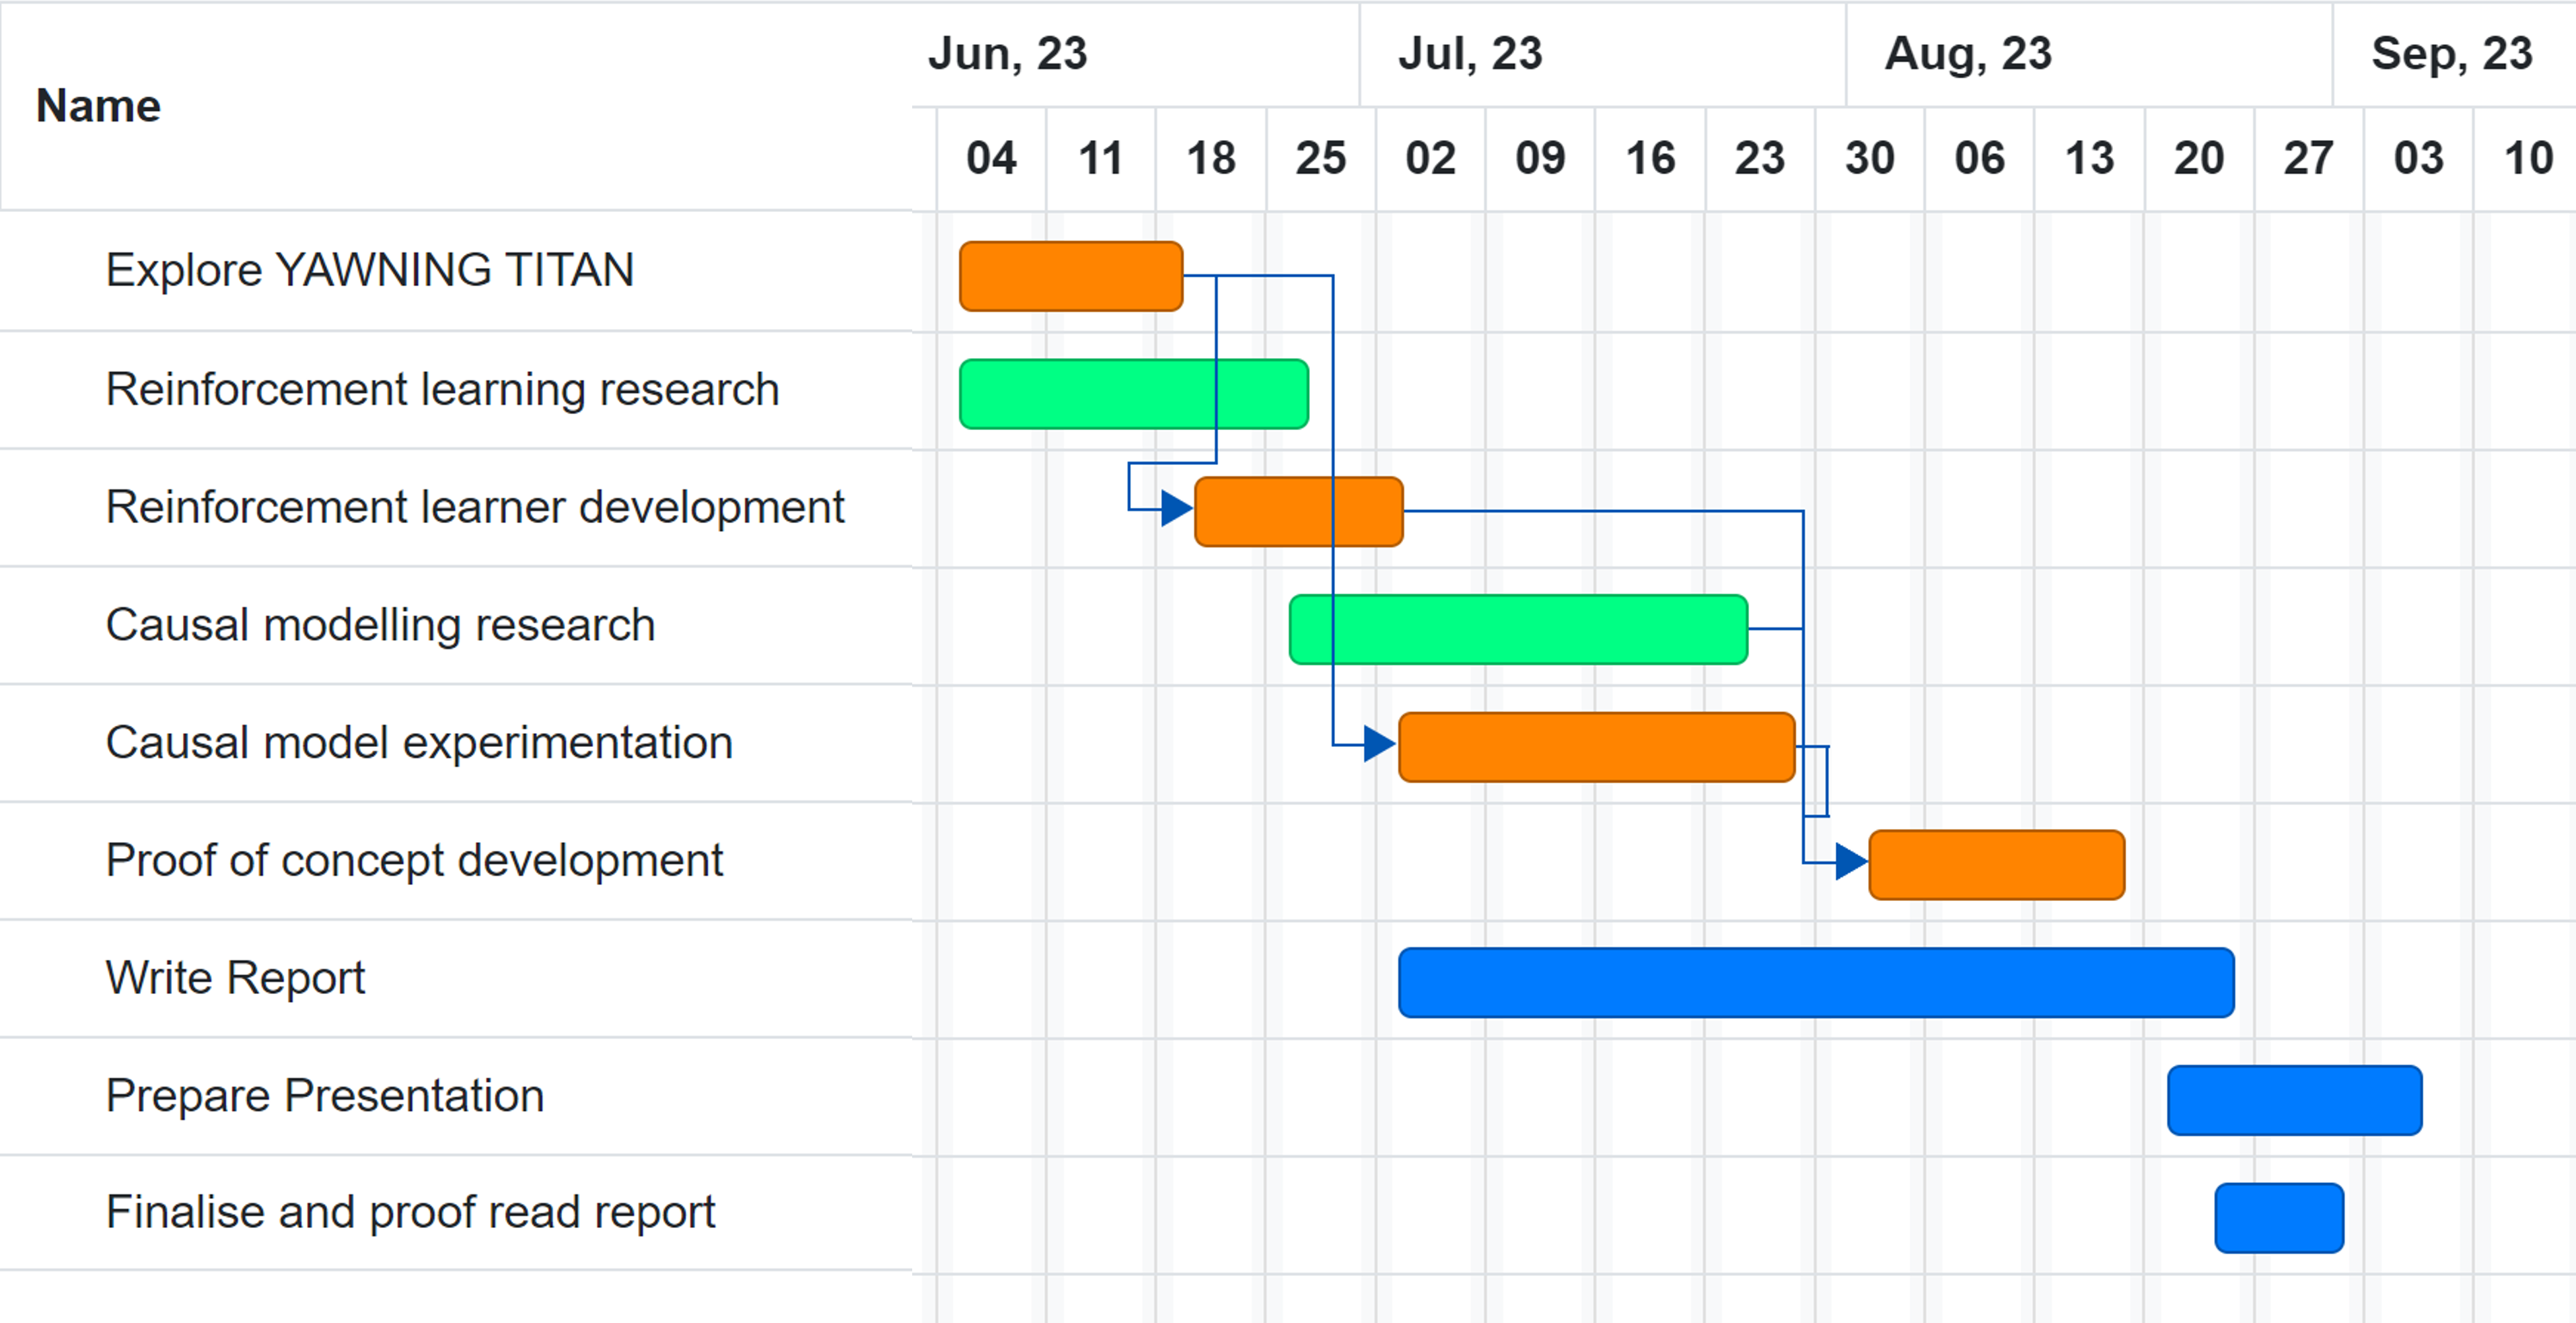
\includegraphics[width=0.99\textwidth]{Images/gantt.png}
    \caption{The Gantt chart breaking down the project workload produced in the preparation stages of the research project. Programming tasks are shown in orange, research tasks in green and writing tasks in blue. The arrows represent dependencies between tasks. Time was kept well and despite challenges, the project progressed almost exactly as expected. }
    \label{fig:gantt}
\end{figure}

\noindent I will now go through each stage of the project in turn, and review the challenges faced and how they were overcome.  

\subsection{Initial agent training}

%learnt SB3 and how to implement algs

 % implemented PPO from scratch, 

% Difficult to get YT up and running
% Spent too long learning about RL methods - could have spent more time on other things. Could have benefitted from more focus for reading


The first challenge faced in my research was to install and use the YT package. Despite seeiming being a relatively simple task, and despite the presence of installation instructions in the documentation \cite{YTdocs}, this proved to be a significant challenge. The powershell commands set out in the setup instructions frequently produced errors, and I struggled to find immediate solutions. As a small-scale and relatively new project (first released in December 2022), there are very few examples of the usage of YT online, making it difficult to troubleshoot. As a result the installation required experimentation with different versions of Python and other dependencies, before the software was able to be used. In addition, a new version of YT was released during the time spent experimenting with the install, which slowed the process further. 

Once functioning, I was able to set up a network in YT with relative ease and used the ability to run through episodes playing as a `keyboard agent' to familiarise myself with the game setup.  This involved acting as the blue agent and choosing actions to defend the network, and allowed me to quickly learn about the actions available and their impact on the system.

Given my relative unfamiliarity with reinforcement learning, the initial weeks of the project were spent concurrently studying the necessary theoretical concepts and implementation details. To do this, I relied on \cite{sutton2018reinforcement}, which provides a thorough grounding on Markov Decision Problems and approaches to training reinforcement learners. From this, I was able to distill the key details presented in Section 2.1 of the technical report. To familiarise myself with state-of-the-art DeepRL algorithms, I completed the `Introduction to DeepRL' course provided by Hugging Face \cite{HFcourse}. This course was chosen specifically as it provided an introduction to Stable Baselines3 \cite{stable-baselines3}, the RL library for which YT was designed to be compatible, and featured practical exercises which enabled me to gain experience implementing a DeepRL algorithms such as DQN \cite{mnih2013playing} and PPO \cite{schulman2017proximal}. Following this course also enabled me to compare DeepRL algorithms and ultimately select PPO for use in my research due to its popularity high performance, despite inherent opaqueness (see Section 2.1 of the technical report). 

However, in hindsight, I feel that I spent too much time researching RL considering that the main goals of my project were not to optimise the performance of an RL agent, but to investigate the factors influencing its decisions. In particular, while completing tasks such as implementing PPO from scratch and reading about multi-agent systems provided a thorough background, many of these details did not make it into the final report. Hence, my project could have benefited from allocating more time to identifying the necessary concepts in RL, and focussing my reading so that I only studied the parts essential for the intended goals. 

Nevertheless, by the beginning of July I was able to successfully train a PPO agent in the YT environment and moved on to the second phase of the project. 

\subsection{Literature review}
After training a DeepRL agent in the YT environment, I began reviewing the literature surrounding explainable reinforcement learning (XRL).

I began reviewing the literature around XRL by reading the papers suggested in the project brief (\cite{madumal2020explainable}, \cite{inproceedings} and \cite{wang2022causal}). I then branched out by examining relevant studies cited in the `related work' sections of these papers, in order to identify influential works in the field. I also found past surveys of XRL related works and XAI in general (including \cite{glanois2021survey}, \cite{heuillet2021explainability} and \cite{wells2021explainable}), so as to gain a broader perspective of the body of research as a whole.

As discussed in Section 3.1 of the technical report, one of the first challenges I encountered was the fact that the research area is still in its infancy, and as a result, there aren't yet unified evaluation metrics for explanation generation methods, or even a consistent definition of what is meant by `explainable'. Hence, studies were difficult to compare, and I had to take extra care to understand the exact aims and achievements of each. I decided to include a discussion of the various uses of the terms `explainability' and `interpretability', and how they can be distinguished, as I feel that this helps to give perspective on the current early state of the body of research, and agreeing on fixed definitions is a key hurdle that needs to be tackled in the field. 

Many surveys, including those mentioned above, propose a taxonomy by which to classify XRL studies. However, none that I encountered seemed satisfactory to organise the papers I had seen. In particular, I found that most proposed taxonomies used categories which do not deterministically divide the methods. For example, in \cite{heuillet2021explainability}, the authors divide post-hoc explanation methods into `saliency maps' and `interaction data'; but saliency maps are generally produced via interaction data, and as claimed in \cite{wang2022causal}, many post-hoc explanation mechanisms for non-image data stem from the saliency map technique proposed in \cite{simonyan2013deep}. Hence, I decided to suggest my own simple taxonomy, explained in Section 3.2 of the technical report and reproduced in Figure \ref{fig:xrl_taxonomy}. 

\begin{figure}[htp]
    \centering
    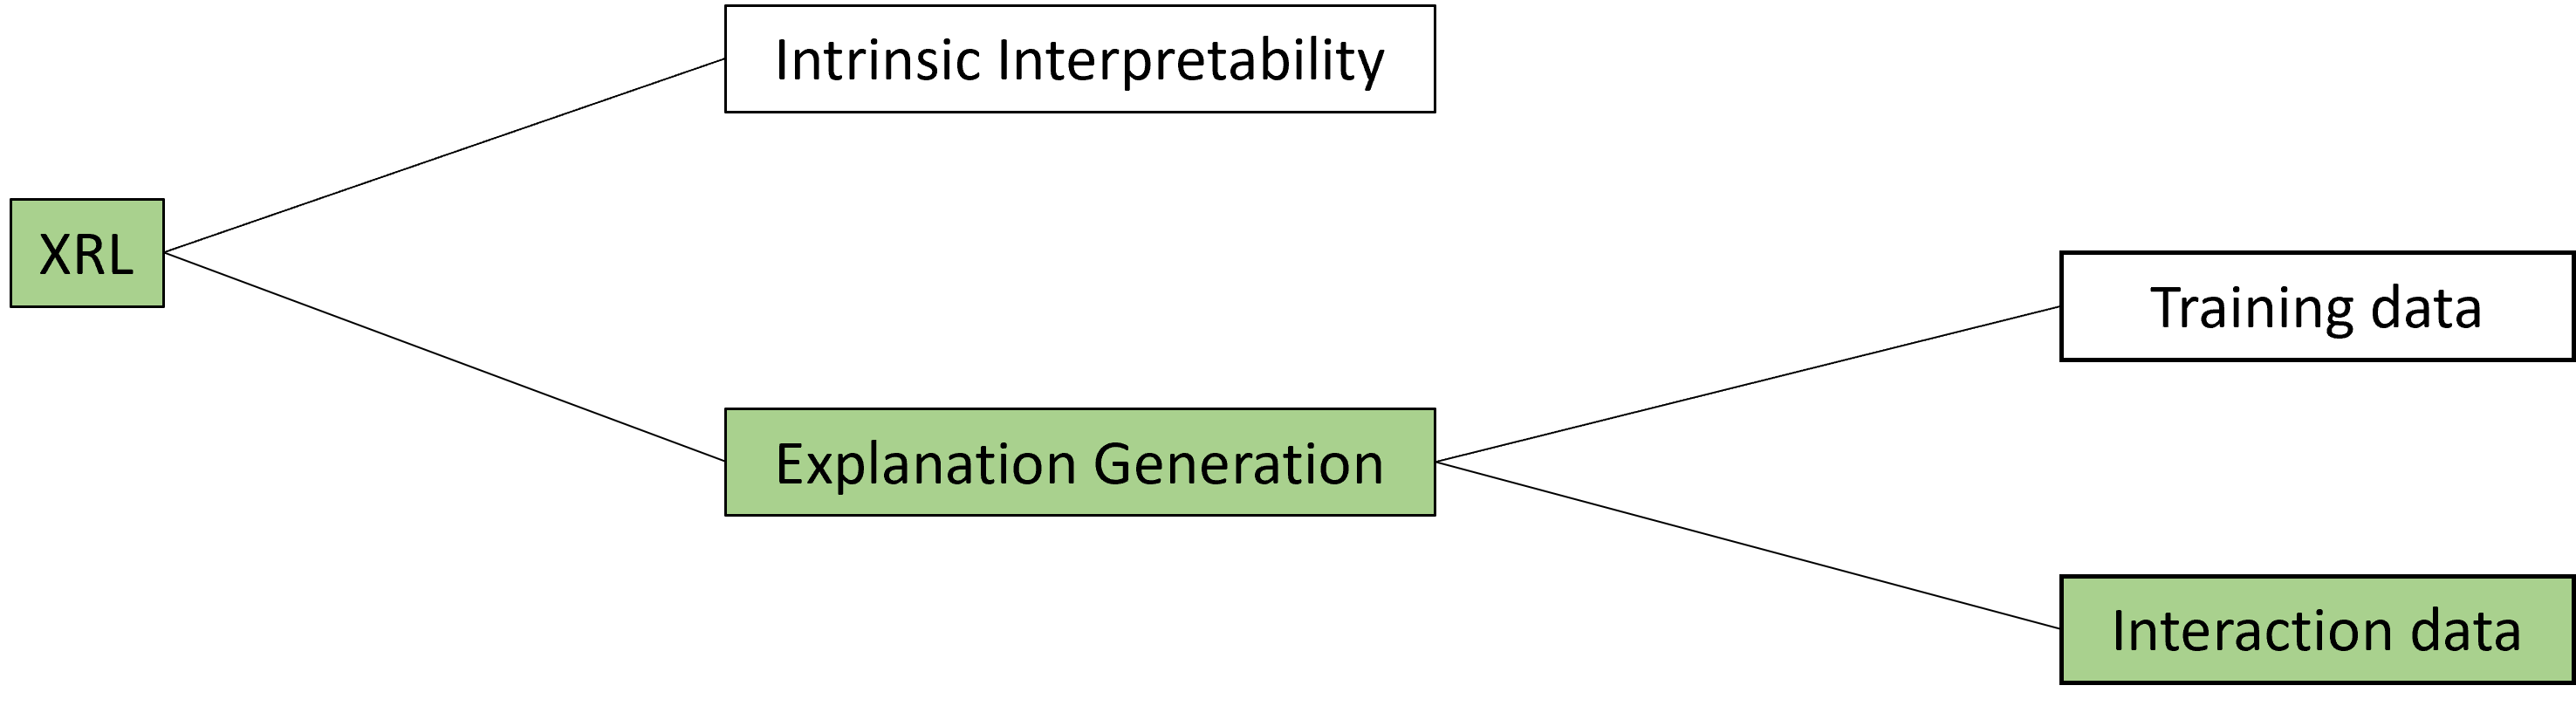
\includegraphics[width=0.8\textwidth]{Images/XRL taxonomy.png}
    \caption{The proposed taxonomy of XRL research reproduced from the technical report. The green indicates the class of the method featured in this research.}
    \label{fig:xrl_taxonomy}
\end{figure}

As in both \cite{glanois2021survey} and \cite{heuillet2021explainability}, I first divide XRL into intrinsically explainable algorithms and explanation generation techniques, in line with my findings about the distinction between `interpretability' and `explainability'. I then categorised the explanation generation techniques according to the stage at which data is collected to train the explanation generation model. This decision was made for two reasons; firstly, the category in which each method fits can be easily determined by examining the details of the proposed method, and secondly it seems valuable to distinguish the stage at which the architecture for the explanation generation technique needs to be in place. In particular, methods trained using interaction data can be used to explain the decisions of agents which have already undergone training, preventing the need for costly retraining. I decided not to investigate or propose further categorisations for intrinsically interpretable algorithms, as I wanted the focus of the literature review to remain on post-hoc explanation generation, in line with the aims of the project. 

When concentrating specifically on causal XRL, I found the current literature sparse, and identified only three key studies; \cite{madumal2020explainable}, \cite{wang2022causal} and \cite{madumal2020distal}. I thus gave a detailed review of each in the technical report to highlight the differences between them and give insight into the current state of the art. 

Since all three reviewed studies provide examples in somewhat `toy' scenarios (Starcraft II, lunar lander, blackjack and a contrived crop irrigation problem), it was difficult to determine a priori how these methods could be applied to the YT environment, which is more complex in terms of the number of variables and causal structure. I decided to first consider the action influence model suggested in \cite{madumal2020explainable}, as this method has shown promise in human studies, whereas the temporal causal model in \cite{wang2022causal} lacks formal evaluation. 

However, I struggled to construct an action influence diagram akin to that shown in Figure 6 of the technical report for even a very simple YT scenario. In particular, while a causal diagram can be constructed between state variables by considering the configuration of YT, the actions available to the blue agent can't be matched to the causal links as elegantly as in the Starcraft II example (\cite{madumal2020explainable}), as the state variables in YT do not have such a simple hierarchical structure. Hence, in order to move forward with the project, I instead focused on adapting the temporal causal graph technique presented in \cite{wang2022causal}. 


\subsection{Causal explanation generation}

\subsubsection{Causal diagram}

Upon considering the causal relationships between the YT state variables, it became immediately apparent that the size of the network considered would need to be reduced dramatically, and the variables included in the observation space carefully considered. In particular, inspecting the options within the YT configuration, one can identify the properties included in the default YT observation space as those in Table \ref{tab: obs space}.

\begin{table}[h!]
    \centering
    \small
    \begin{tabular}{ | m{0.22\textwidth} | m{0.55\textwidth}| m{0.1\textwidth}|} 
      \hline
       \textbf{Property} & \textbf{Description} & \textbf{Size}\\ 
      \hline
         Node connections & An adjacency matrix representing the connections between the nodes in the network & $N^2$ \\ 
      \hline
         Node compromised status & A binary indicator representing whether each node is compromised & $N$ \\ 
      \hline
         Node vulnerability score & A value in $[0,1]$ for each node representing its susceptibility to attack & $N$ \\
      \hline
         Average vulnerability & The mean value of the node vulnerability scores & 1 \\ 
      \hline    
         Graph connectivity score & The proportion of possible node connections which are present & 1 \\ 
      \hline
         Attack sources & A binary indicator representing the nodes from which an attack has previously been launched & $N$ \\ 
      \hline
         Attack targets & A binary indicator representing the nodes which have previously been attacked & $N$ \\ 
      \hline
         Entry nodes & A binary indicator representing whether each node is a designated entry node & $N$ \\ 
      \hline
         High value nodes & A binary indicator representing whether each node is a designated high value node & $N$ \\ 
      \hline
         Red agent skill & A value in $[0,1]$ used in the calculation of the success probability of attack & 1 \\ 
      \hline
      
    \end{tabular}
    \caption{The properties which make up the default YT observation space, and their respective sizes. Here $N$ denotes the number of nodes in the network.}
    \label{tab: obs space}
\end{table}

My initial PPO agents were trained using an 18 node network, and using Table \ref{tab: obs space}, this yields an observation space of 435 variables! Hence much discussion was had in order to select the variables which would be most valuable to remain in the observation space. The aim was to decide on the minimal set of variables which still provide an interesting RL environment and allow the agent to learn a meaningful policy, resulting in the selection of the node connections, vulnerability scores, compromised status and the special node types (entry or high value). Average vulnerability and graph connectivity score were removed as there is a redundancy in information when individual node connections and vulnerability scores are also available. An observation of the red agent's skill was removed as it was chosen that this would remain fixed between episodes in order to simplify the causal structure. Attack sources and targets were removed as these only provide additional information in the form of past events and so were not deemed as important as current state variables such as node vulnerability scores and compromised status. These reductions resulted in the final observation space described in Section 4.2.2 of the technical report. The size of the network was also reduced to just 5 nodes, leading to an observation space of size 45.

The observation space can be altered in the `game mode' setup in the YT GUI, and so I made the necessary changes and trained a PPO agent using the new 5 node network. However, upon inspecting an evaluation episode, I found that the observation matrix was of size 54. This observation matrix was also simply an array of 54 values with no indication as to which properties of the network each corresponded to. Unfortunately, the YT documentation is limited and does not give information about the observation space. Thus, considerable time was spent reading through the source code in order to solve these issues. It eventually transpired that the observation matrix was automatically padded in case the deceptive node capability (where the blue agent can add additional nodes to the network) was enabled, resulting in the inflated size. I was able to remove this padding, and use the source code to identify the order of the variables in the observation matrix to produce the output shown in Figure 11 of the technical report. 


\begin{figure}[htp]
    \centering
    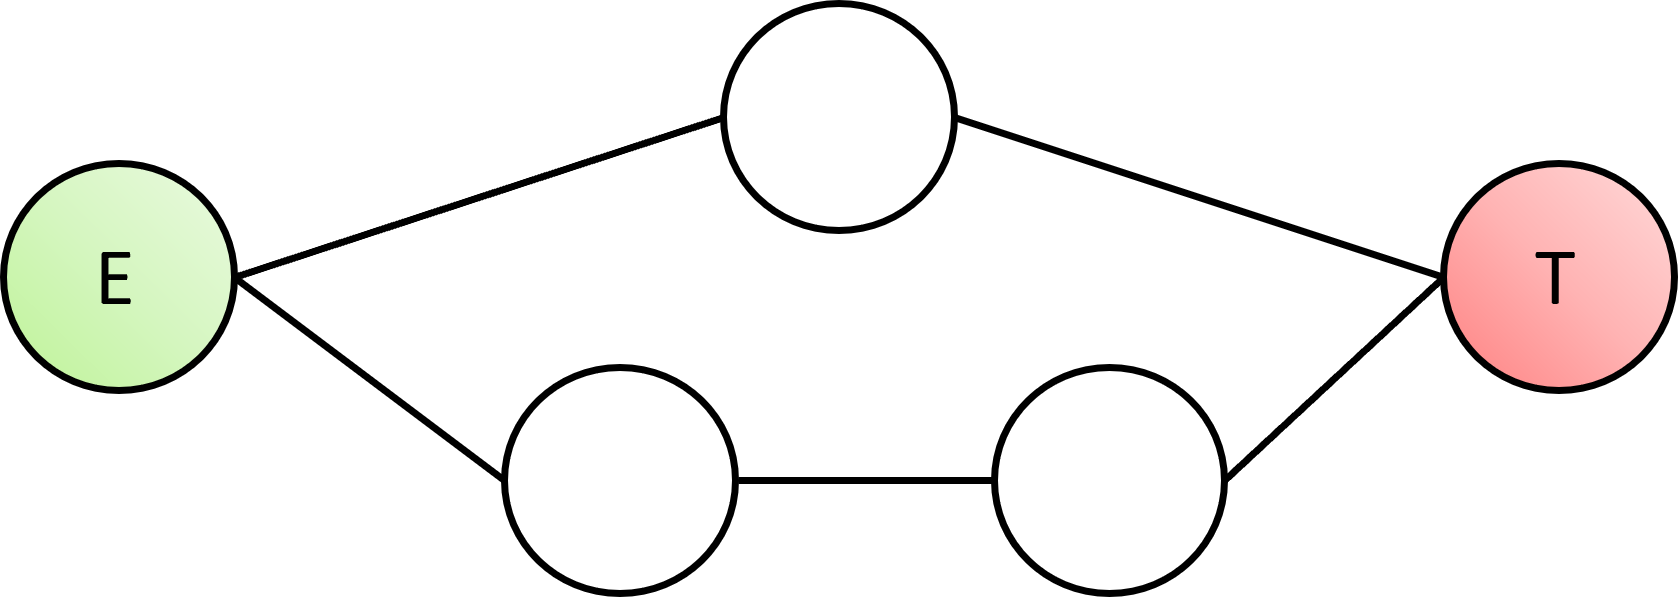
\includegraphics[width=0.6\textwidth]{Images/Initial 5pc.png}
    \caption{The initial 5 node network configuration used when considering causal explanations. The green node represents the entry point, and the red indicates the high value target. This setup was chosen to study the factors influencing the RL agent's decisions to defend either path to the target node. However, this configuration doesn't provide enough distance between entry and target for effective training; the game is `too easy' for the red agent to win.}
    \label{fig:linear_5PC_diagram}
\end{figure}

I initially considered the topology shown in Figure \ref{fig:linear_5PC_diagram} for the 5 node network. This was chosen so that there were multiple attack paths from the entry to target node, as it was deemed to be interesting to consider the factors that influenced the blue agent to defend either path. However, upon training a PPO agent on this network, it became apparent that `game' had become too easy for the red agent to win. In particular, the tensorboard output indicated that the RL agent was not able to effectively train, as the episodes were ending before the blue agent was able to collect rewards. To combat this, the network topology was changed to the linear network described in Section 4.1 of the technical report in order to provide the maximum distance between the entry and target nodes whilst limiting the number of nodes to preserve the simplicity of the causal diagram. Further, the default YT reward function gives a reward of 100 for a blue agent `win' and -100 for a blue agent `loss', and this was altered to the reward function described in Section 4.4 of the technical report. This change reduced the penalty for `closer losses', meaning that a smaller negative reward was obtained when the episode had lasted longer, providing more diversity in rewards to encourage effective training. The above changes were made following much experimentation, during which I also tried removing the red agent's ability to use zero-day attacks and varying the initial node vulnerabilities, however these alterations made little difference.

Up to this point, I had been using the default action space provided in YT, which includes the ability to isolate a node from the network by removing all connections to it. Unfortunately, I now had the opposite problem; the blue agent quickly learnt to defend the network by immediately isolating node 1, so that the red agent was not able to make any progress in the network. Whilst this is clearly an effective way to defend such a small network, the actions following the isolation have little importance on the success of the blue agent, and so it is not interesting to consider the causes of such choices. Thus it became apparent that I would need to carefully consider the action space available to the blue agent. After much trial and error, I settled on the action space presented in Section 4 of the technical report, which allows both proactive and reactive actions, whilst limiting the blue agent's abilities enough to provoke diverse and interesting episodes. I then further refined the balance in the game setup by experimenting with different values for the red agent's skill level, as shown in Section 4.3 of the technical report. 

Once I had created a balanced reinforcement learning scenario, I was then able to produce a temporal causal diagram inspired by those in \cite{wang2022causal}, presented in Section 5 of the technical report.   


\subsubsection{Importance calculations}

After producing the causal diagram, the next task was to adapt the feature weighting calculations in \cite{wang2022causal} for use in the YT environment. In this paper, the authors quantify feature importance by subtracting the true action from the action taken in a counterfactual instance in which the state features were altered. However, the authors don't give details on how they performed this subtraction; in general, finite action spaces don't have an inherent ordering and so subtracting actions doesn't have an obvious meaning. In the YT scenario used in this research, the action space consists of 10 categorical actions encoded as the integers 0-9; subtracting these values would be meaningless. What we are really interested in is whether the action changed, so I first considered using an indicator function representing whether the counterfactual action differed from the true action. However, this does not capture the stochasticity of the PPO policy and YT environment, and can be misleading if the approximation for the structural equations incorrectly predicts the counterfactual action. Hence, I instead chose to predict the probability that each action was taken in the counterfactual instance, and transform the actual action into a vector using one-hot encoding to enable subtraction. I decided to use the $L_2$ norm to quantify the distance between the two vectors so as to apply a heavier weighting to differences closer to 1, as these imply a more certain change in action. If I had more time, I would like to have experimented with different metrics to quantify the change in action and determine the effect this has on the insights derived from the feature weightings.

Predicting the counterfactual actions required  approximations of the structural equations defined in Section 5 of the technical report. Inspired by the use of regression techniques in both \cite{madumal2020explainable} and \cite{wang2022causal}, and due to the fact that the YT observation space consists of a mixture of binary and continuous features, I chose to use logistic regression. However, due to the delays caused by the problems outlined in Section 3.3.1 of this report, this decision was made in haste. Thus if the project were to be extended, I would spend time comparing classification techniques for this task in order to maximise the accuracy of the counterfactual predictions. 

To train the logistic regression models, I first used a dataset of post training interaction episodes, as suggested in \cite{wang2022causal}, and evaluated the model fit using a 90/10 train/test split. This showed 99\% prediction accuracy and so I proceeded with the feature importance calculations. However, plotting the feature importances yielded strange and inconsistent results; very similar states often had wildly differing associated feature importance values. Upon closer inspection, I realised that in the collected interaction data episodes, the blue agent was so effective that there was rarely a case where more than one node was compromised at any one time. Hence, the model was not able to accurately predict the result of counterfactual instances in which multiple nodes were compromised. I tested this theory by comparing the model's predictions to the trained RL agent's predicted actions for randomly generated instances of the state space, and obtained an accuracy of only 23\%. Thus, I instead created a training dataset for the regression model by drawing random values from the possible state space and allowing the PPO agent to predict the action it would take. The environment was then stepped to obtain the next state. This meant that the model for predicting the counterfactual actions was exposed to a broader range of agent behaviour during the training, resulting in more accurate predictions. 


\subsection{Technical issues}

During this project, I encountered many technical issues with YT. In particular, installing further modules often caused YT to stop working, meaning that it had to be deleted and reinstalled. Towards the end of the project, I also encountered a bug when altering game modes in the YT GUI, which prevented the use of any configuration other than the default. Further, the documentation for YT is very limited, resulting in the need to examine the source code to determine the result of certain features. This made experimentation with the software difficult and time-consuming. For example, at one stage I experimented with the feature `natural spreading'. In the documentation, \cite{YTdocs}, it states that this allows red agent control of the network to spread from a compromised node to a neighbouring node with a set probability in each turn. However, examining episodes with this feature enabled shows strange behaviour. In particular, as shown in Figure \ref{fig:YT strange}, this sometimes resulted in the compromise of nodes not connected to any entry or previously compromised nodes. 

\begin{figure}[htp]
    \centering
    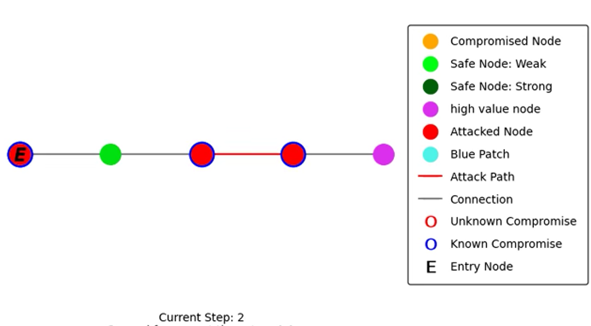
\includegraphics[width=0.6\textwidth]{Images/YT_strange.png}
    \caption{A screenshot of a gif produced from an evaluation episode of a trained RL agent in YT. In this scenario, the `natural spreading' option has been used, which the documentation implies allows a red compromise to spread to a neighbouring node with a set probability in each turn. However, we can see that nodes 3 and 4 are compromised in turn 2, despite these being connected to neither an entry node nor a previously compromised node. }
    \label{fig:YT strange}
\end{figure}


Looking back on the project, these issues with YT, combined with the huge number of configuration parameters perhaps imply that YT was not the most appropriate choice of cybersimulator for this project. The flexibility of YT provides an interesting environment for comparing the behaviour of defensive RL agents in different settings, however for my purposes, the complexity of the software only seemed to hinder progress. I ended up simplifying the YT scenario to the point that perhaps it would have been prudent to have instead set up a small network defence scenario from scratch. In that case, the structure of the MDP, including the state space, impact of the available actions, transition probabilities and  reward function, would have been clear from the start, and I would have spent less research time reading source code in order to identify these parts. Nevertheless, learning to problem solve within YT has provided a valuable learning experience and I have gained skills in working with unfamiliar code and new software.  

% too complex to be worth it when all i want is a simple causal scenario  
% YT very opaque, hard to find anything

% Difficult to interpret output of episode replay - actions output as numbers which change when agent retrained - have to match up using `info' parameter. 

% Strange behaviour -- evidence with screenshot

% Bugs at end of project 

\section{Limitations and further work}

The two greatest deficiencies of the method proposed in this project are the lack of formal evaluation and limited scalability. Both of these limitations were identified as common to the majority of XRL studies during the literature review, yet are vital to broaden the applicability of explanation generation techniques to real-life settings, particularly high stakes environments such as in cyber security. Thus, if the project were extended, one of the immediate goals would be to perform a targeted human study to assess the efficacy of the proposed method for aiding cyber security professionals' understanding of the decisions made by an RL agent. This could be assessed using task prediction and explanation satisfaction, as is done in \cite{madumal2020explainable}, although the format in which the explanations are presented to the participants would need to be carefully considered. In particular, it may be useful to consider the use of NLP templates, as used in \cite{madumal2020distal}, in order to make the information easier to interpret. 

Given more time, I would also investigate the scalability of the method by applying it to larger and more complex network topologies and observation spaces. Further, YT has many additional options not considered in this research which could make the environment more representative of real-life scenarios, such as the ability to make the compromised status of the nodes partially obscured. For example, the environment can be configured so that the blue agent does not have a full view of the red agent's presence in the network, and can gain more information via a `scan' action. This is a better reflection of true cyber defence scenarios, in which intrusions aren't always immediately apparent. However, the more complicated the environment, the harder it becomes to derive an accurate causal model representing the system dynamics. Thus, in order to truly enhance the scalability of the explanation generation method, it is necessary to investigate how causal discovery techniques, such as those discussed in \cite{glymour2019review}, can be incorporated to relax the assumption of a pre-determined causal structure. 

Additionally, the causal model used in this approach assumes a static network structure. This is in contrast to real-life networks, in which there are often changes in connectivity such as new nodes being added or broken connections being severed. Hence, it would be interesting to investigate how the causal model could be modified to encompass dynamic networks, where the entry nodes, targets and network topology change during the episode.

There is also space for further work refining the importance weighting calculations in Section 5 of the technical report, such as determining the effects of variations in the mechanism used to quantify the distance between the counterfactual prediction and true action, as well as optimising the classifiers used to approximate the structural equations, as discussed in Section 3.3.2.


% Where I would have liked to have taken the project if I had more time/ resources / brains

% More complex network topologies, incorporating more agent actions,...

% Vary weighting calculation methods - would really like to have done a comparison of classification methods to determine the best way of learning structural equations

% What if topopology was dynamic?

% Limitations in XRL - human studies, scalability (causal diagram requirement)

\section{Key takeaways}
In summary, this research was successful in terms of the project aims of training a reinforcement learner in the cybersimulator YAWNING TITAN, surveying the literature surrounding explainable reinforcement learning and developing a proof of concept using causal models to give insight into the decisions made by the trained RL agent. However, the proof of concept proposed only considered a highly specific, simplified network defence scenario and so there is much further work to be done to broaden the applicability of the technique. Further, it was found that due to the large number of parameters and difficulty in using YT, it may not have been the most appropriate choice of software for the project. 

%  What did my paper contribute and what did I learn 
%wrap up by summarising points made

\pagebreak


\section{References}
%\bibliographystyle{unsrt}
%\bibliography{report}


\printbibliography[heading=none, stylename = plain]

\end{document}
